\chapter{Design}

\section{Architecture overview}

The Connectivity Manager is logically located between the EMM and the cloud infrastructure and provides the following two functionalities:
\begin{itemize}
\item \textbf{Optimal Instance Placement:} During the deployment of a stack an algorithm chooses where individual instances are placed within the cloud infrastructure.
\item \textbf{Service-Level-Agreement enforcement:} Depending on the services that an instance provides to the rest of the stack, certain requirements for its network performance need to be fulfilled.
\end{itemize}

\begin{figure}[H]
\centering


\includegraphics[width=0.5\textwidth]{images/design/functional_architecture}

\caption{High-level architecture of the Connectivity Manager}
\end{figure}

The \textit{Instance Placement Engine} determines if and where the instances should be deployed. It does so by comparing the current utilization and capacity of the available compute nodes within the availability zone.

The \textit{QoS Manager} enforces different QoS policies based on the type of service that the instance is grouped in. A guaranteed and maximum bit-rate for the network port of an instance can be set. This way a certain network performance can be insured.

\section{Connection between Manager \& Agent}

The Connectivity Manager and Agent are two separate applications that communicate using a ReST API. 

\begin{figure}[H]
\centering

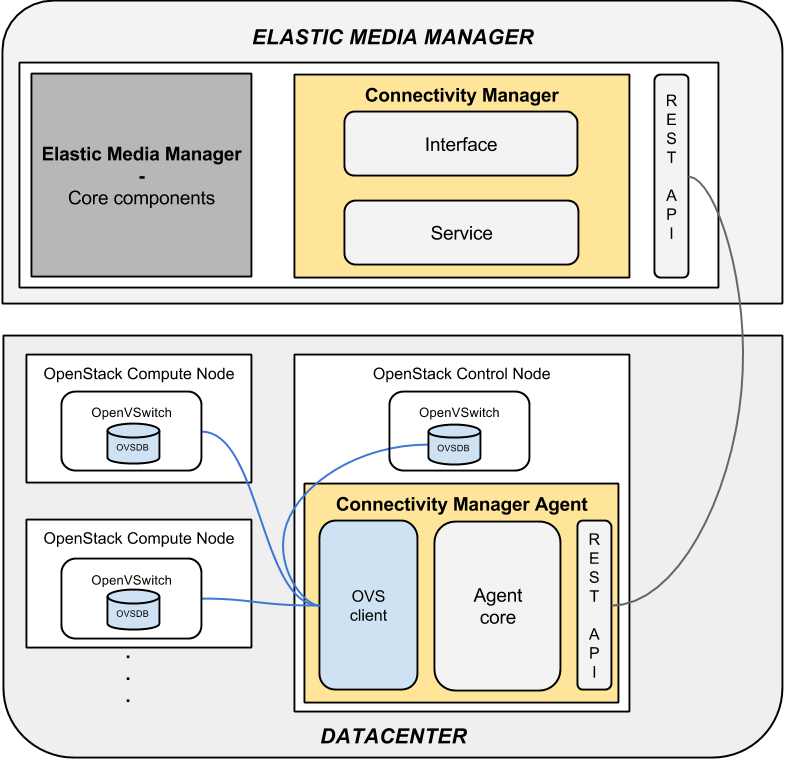
\includegraphics[width=0.6\textwidth]{images/design/modular_architecture_cm_cma}

\caption{Minimized architecture of the Connectivity Manager and its integrations}
\end{figure}

This design was chosen first of all because the Connectivity Manager is integrated in the EMM, which is required to be placed anywhere outside of the data center. Second of all the Connectivity Manager Agent needs to  the OVSDB on the compute nodes and consequently needs to be within the internal management network of the OpenStack infrastructure.

The sequence diagram below displays the work-flow that the CM passes during the run-time.

\begin{figure}[H]
\centering

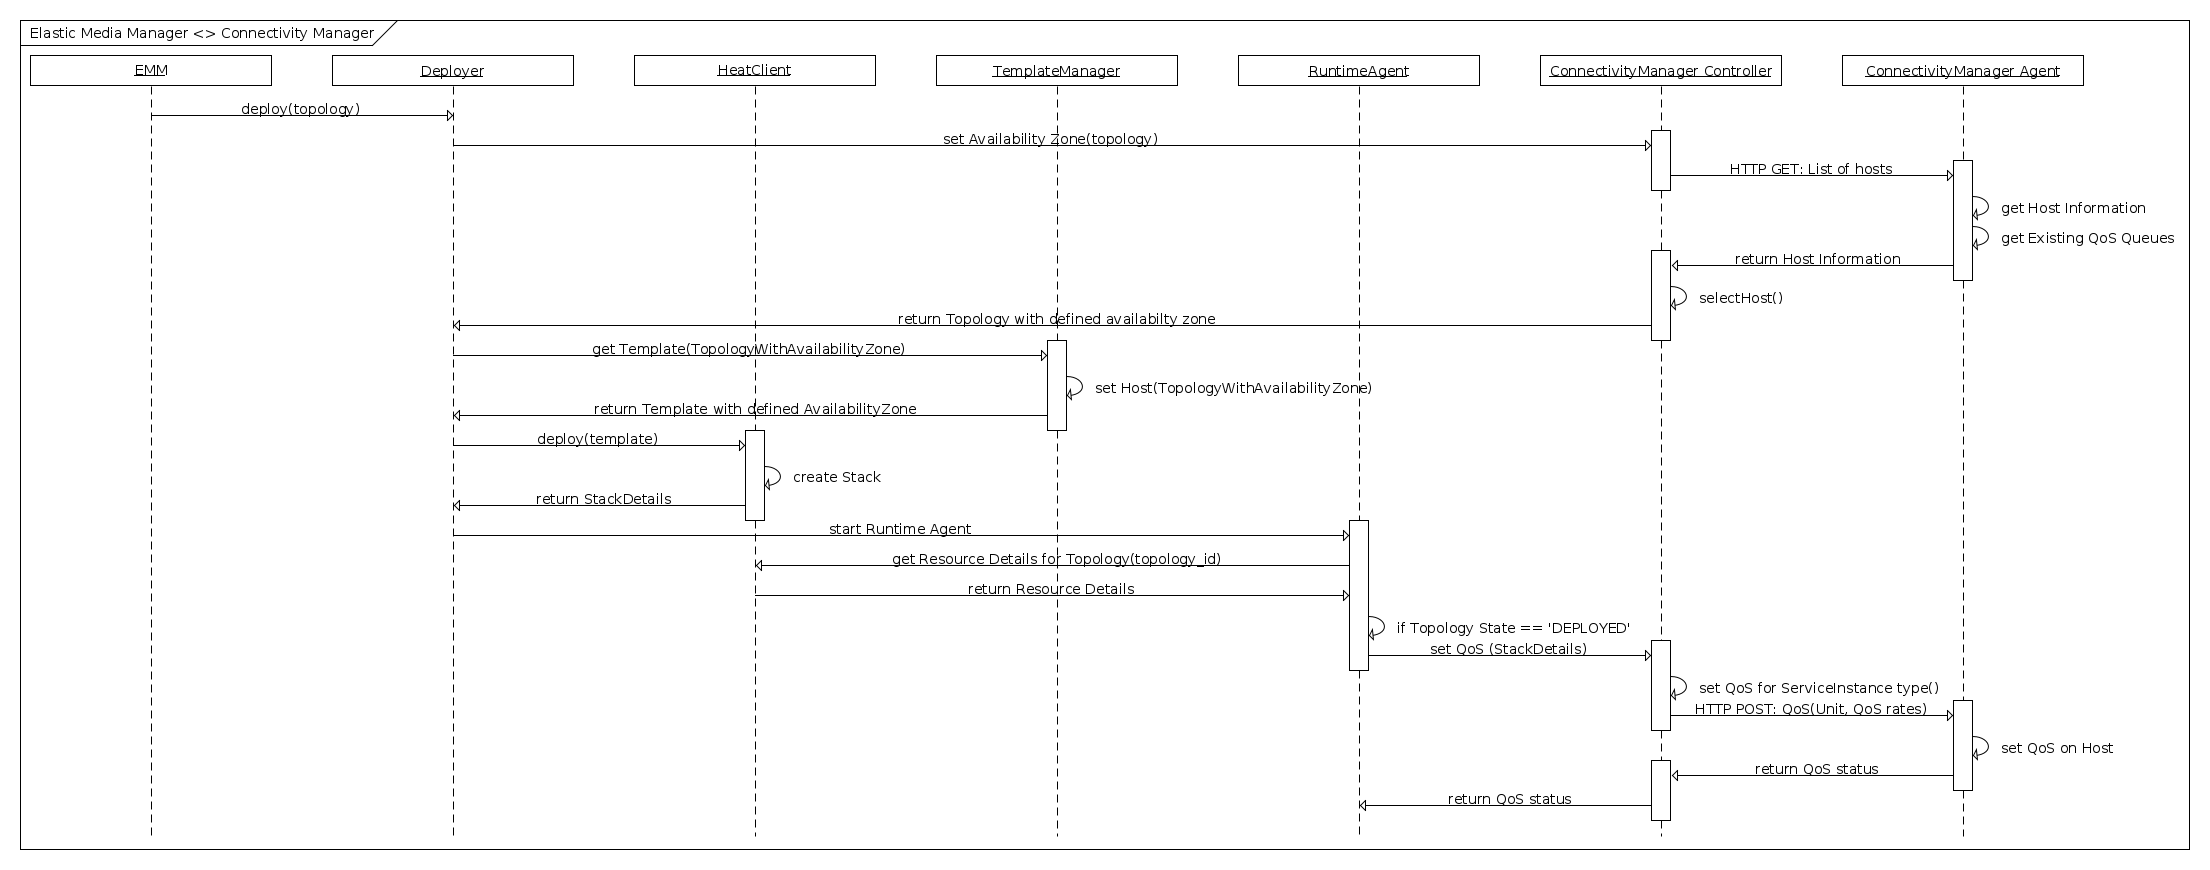
\includegraphics[width=0.9\textwidth]{images/design/sequence_diagram}

\caption{Workflow: Deployment of stack \& Assignment of QoS policies}
\end{figure}

As visible in the above figure, the Connectivity Manager receives the Topology object that contains a description of the configuration and specifications of the whole cloud. For the placement decision the CM to needs to get the information about the current state of the infrastructure. This exchange with the CM Agent occurs through the given API. Upon reception of that data, the placement algorithm sets the availability zone for each instance within the topology. The topology is then converted into a Heat template by the Template Manager. Once the template got deployed by the Heat Client a runtime agent starts. The purpose of the runtime agent is to continuously check the state of the stack. Once the stack has reached the 'DEPLOYED' state, the runtime agent requests the CM to set the QoS policies according to previously configured values. This configuration is subsequently transmitted to the CM Agent whose task is then to enable it on the according ports of the instances within the Open vSwitch.


\section{Design of Connectivity Manager}

The design of the Connectivity Manager is based on the framework that already exists in the Elastic Media Manager.

It consists of a highly dynamic Factory, abstract Interfaces and the actual implementation as a Service.
The Factory Agent reads a configuration file in which the class name of the service for the according interface is defined. It then instantiates a instance from that given class. This means it is easy to replace the actual implementation while the interface to the other components remains identical.

\begin{figure}[H]
\centering

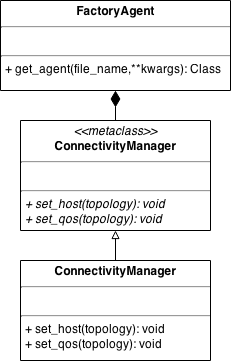
\includegraphics[width=0.2\textwidth]{images/design/cm-emm_interface_classes}

\caption{Class diagram: Metaclass (Interface) and implementation (Service) instantiated by Factory Agent}
\end{figure}

The Connectivity Manager interface and service only contain the methods that are later called by the Elastic Media Manager. However additional helper classes are needed in order to provide the appropriate configuration and the communication with the Connectivity Manager Agent, as shown in the next figure.

\begin{figure}[H]
\centering

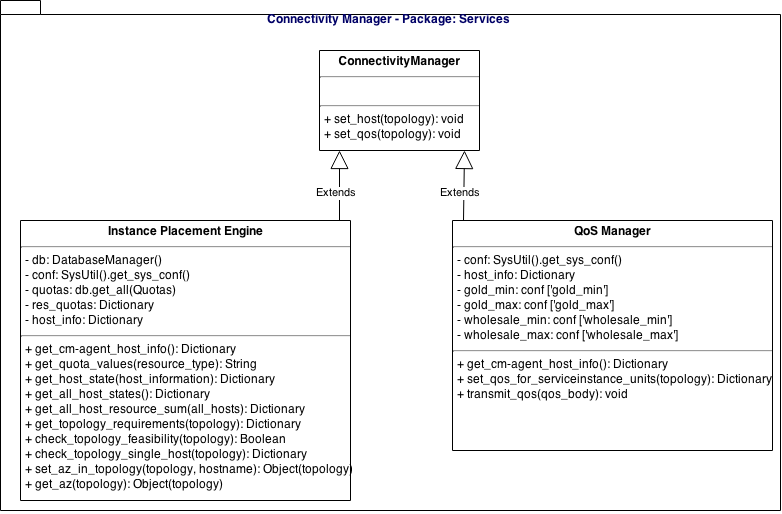
\includegraphics[width=0.6\textwidth]{images/design/cm_class_diagram}

\caption{Class diagram: Connectivity Manager service and its helper classes}
\end{figure}

The topology that is created by the EMM and contains the required resources for the stack are visible in the next diagram.

\begin{figure}[H]
\centering

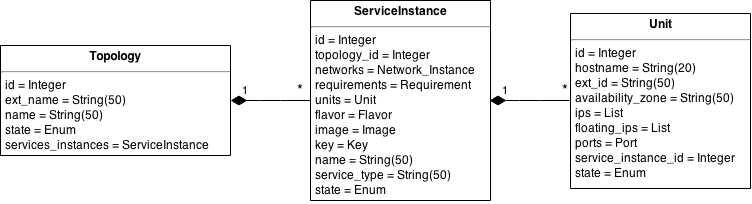
\includegraphics[width=0.9\textwidth]{images/design/cm_topology_object}

\caption{Deployment: Topology object from EMM}
\end{figure}

This object is handed over to the CM during the deployment phase. The topology can contain multiple Service Instances, which defines general parameters such as which networks the underlying instances need to be connected to, the flavor wherein the resources (e.g. amount of RAM \& CPU) are specified, the image that contains the operating system and additional software packages and the key that is needed to establish a console connection via SSH.

Each Service Instance can contain multiple Units (instances). Among others it contains parameters like IP addresses, the availability zone that it gets deployed on and the external ID which is unique across the whole infrastructure.



\subsection{Algorithm for Instance Placement}

The following section describes the algorithm that is used for setting the availability zone for the instances, and thus placing them in the most advantageous way based on the project requirements.


Each tenant has a set of quotas which limit the resource usage within the OpenStack infrastructure. Limitations can be made based on the following resource types (excerpt): Amount of instances, vCPU's, RAM, Floating IP addresses and fixed IP addresses.

Considering the requirement to have optimal connectivity between individual instances, it is preferable to position them on the same compute node, given that its resources allow this.

\begin{figure}[H]
\centering

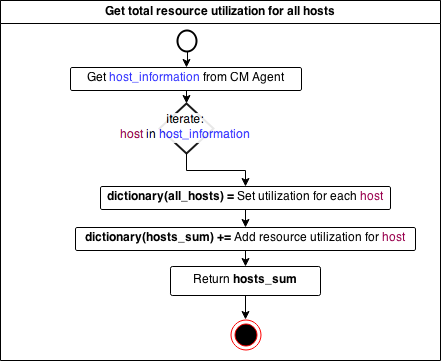
\includegraphics[width=0.7\textwidth]{images/design/cm_get_host_utilization}

\caption{Check resource utilization of hosts}
\end{figure}

\begin{figure}[H]
\centering

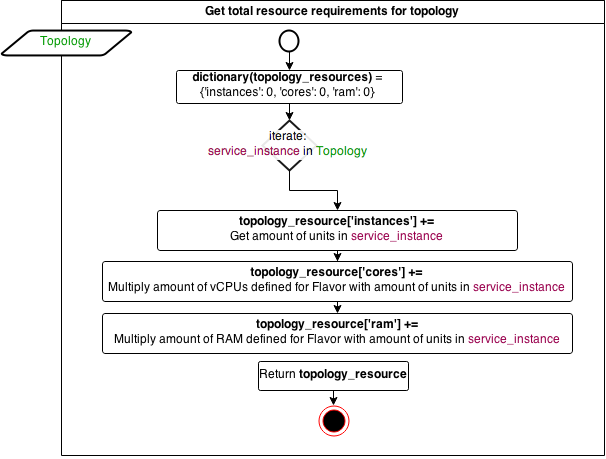
\includegraphics[width=0.7\textwidth]{images/design/cm_get_topology_requirements}

\caption{Get total amount of required resources for topology}
\end{figure}


\textbf{Step 1: Check if Topology is within the limitations of the Quota and currently available resources on the overall hosts.}

\begin{figure}[H]
\centering

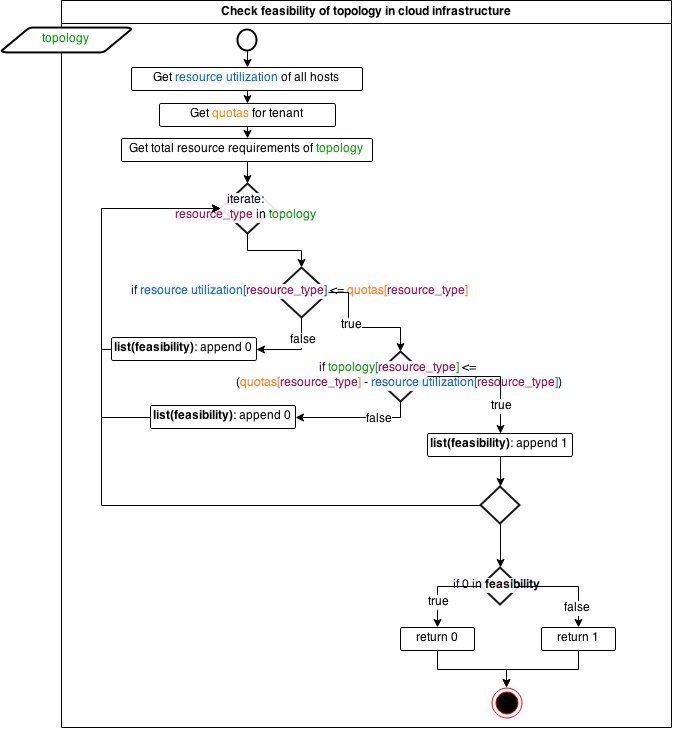
\includegraphics[width=0.7\textwidth]{images/design/cm_feasibility_check}

\caption{Check if deployment is feasible within infrastructure resources and tenant quota}
\end{figure}


\textbf{Step 2: Check whether the Topology can be deployed on a single host.}

\begin{figure}[H]
\centering

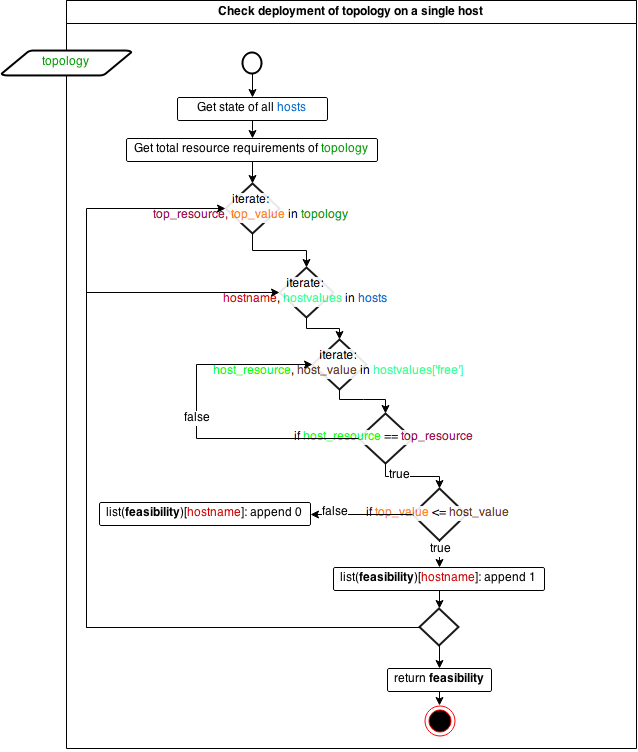
\includegraphics[width=0.7\textwidth]{images/design/cm_single_host_check}

\caption{Check if topology can be deployed on a single host}
\end{figure}


\textbf{Step 3: Set selected host as availability zone for each Unit.}

\begin{figure}[H]
\centering

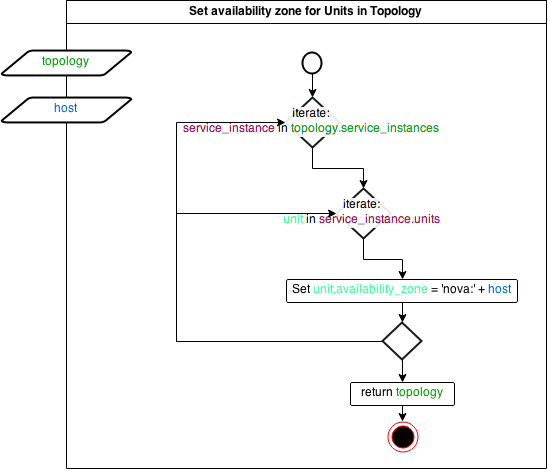
\includegraphics[width=0.7\textwidth]{images/design/cm_set_az_topology}

\caption{Set the availability zone for each Unit}
\end{figure}


%\textbf{Step 3: Check on which host the biggest proportion of the Topology can be deployed.} %


\newpage
\section{Design of Connectivity Manager Agent}

\begin{figure}[H]
\centering

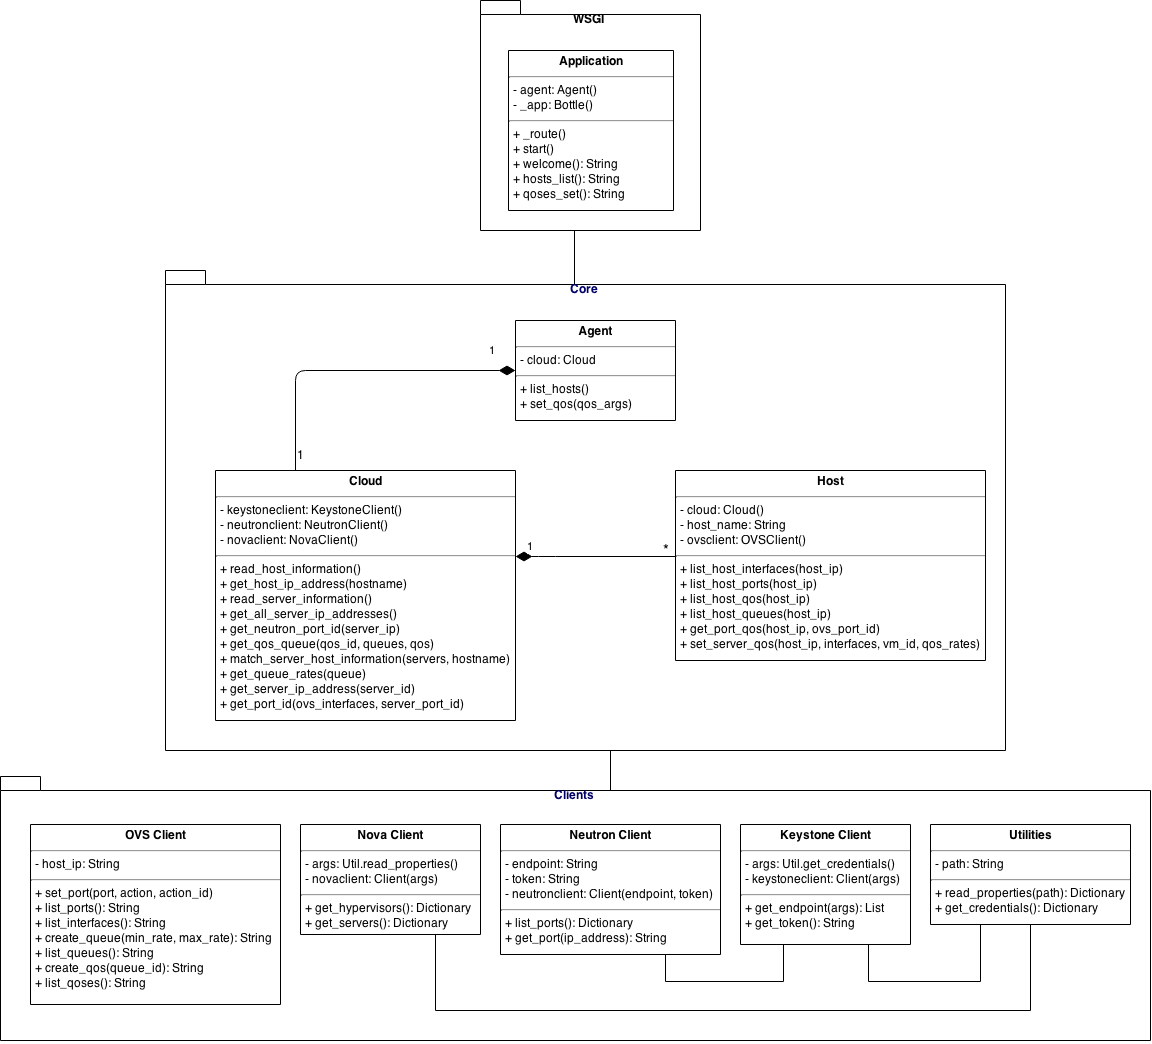
\includegraphics[width=0.7\textwidth]{images/design/cm_agent_class_diagram}

\caption{Class diagram: Connectivity Manager Agent - Core package}
\end{figure}


\begin{figure}[H]
\centering

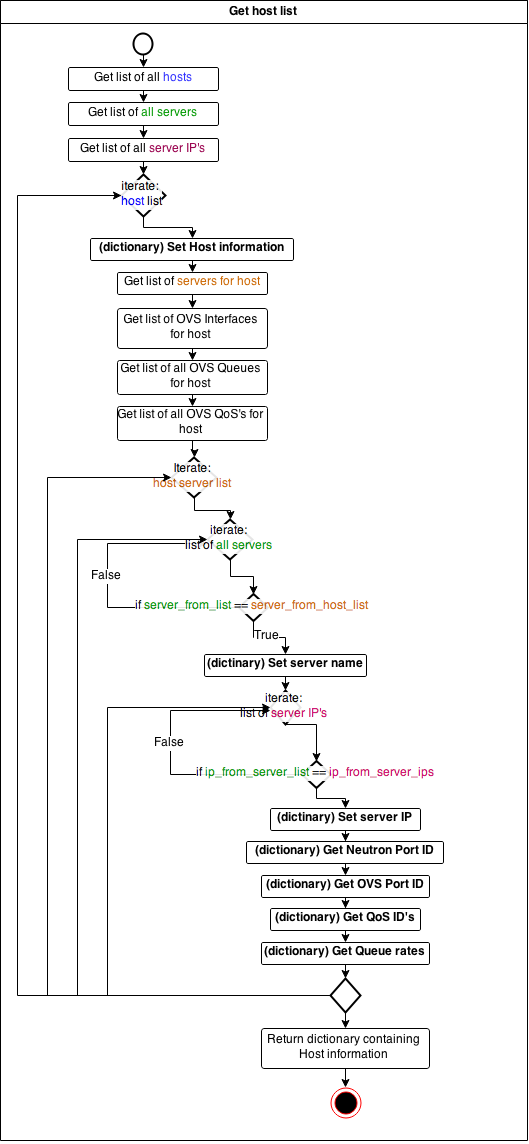
\includegraphics[width=0.7\textwidth]{images/design/activity_host_list}

\caption{Activity diagram: Get list of hosts}
\end{figure}

\begin{figure}[H]
\centering

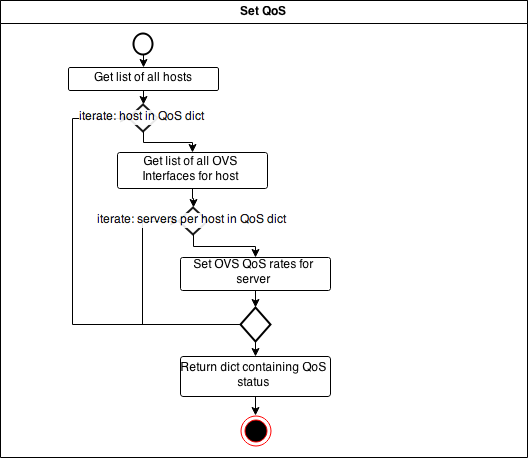
\includegraphics[width=0.7\textwidth]{images/design/activity_set_qos}

\caption{Activity diagram: Set QoS rates for all servers}
\end{figure}

\begin{figure}[H]
\centering

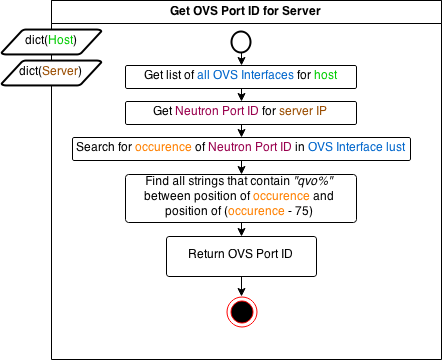
\includegraphics[width=0.7\textwidth]{images/design/activity_get_ovs_port_server}

\caption{Activity diagram: Get OVS Port ID for server}
\end{figure}

\begin{figure}[H]
\centering

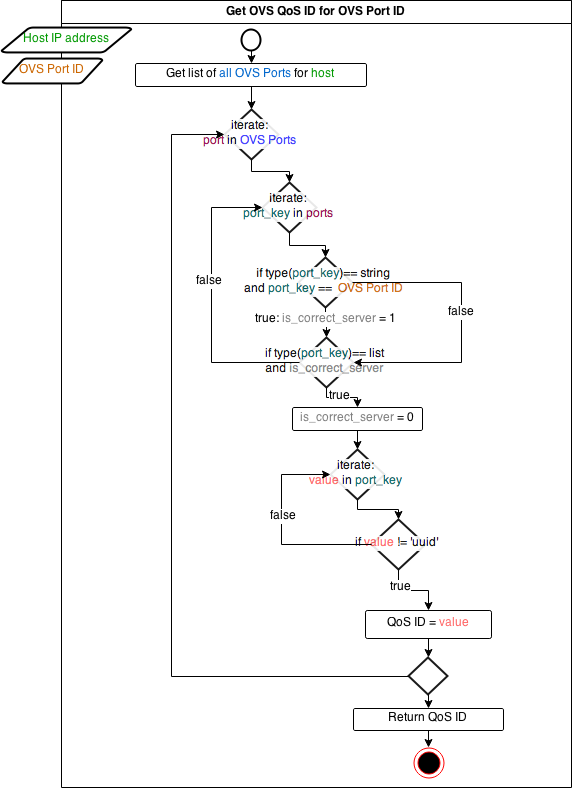
\includegraphics[width=0.7\textwidth]{images/design/activity_get_qos_id_for_ovs_port}

\caption{Activity diagram: Get QoS ID for OVS Port}
\end{figure}





\section{Conclusion}